\documentclass[titlepage,12pt,twoside]{article}

%\pagestyle{headings} 
\pagenumbering{arabic}
\textheight240mm            \textwidth150mm  \parskip0pt plus3pt
\marginparwidth22mm  \marginparsep3mm
\oddsidemargin4.6mm   \evensidemargin4.6mm  \topmargin-20mm
\setcounter{secnumdepth}{5}  % = Nummerierung vertiefen *
\setcounter{tocdepth}{4}		

 % = Aufnahme von paragraph und subparagraph in das Inhaltsverzeichnis *

\usepackage[latin1]{inputenc}
\usepackage[T1]{fontenc}
\usepackage[ngerman]{babel}
\usepackage{amsmath}
\usepackage{verbatim} %Für Blockkommentare
\usepackage{wrapfig}
\usepackage{multicol}
\usepackage{graphicx}
\usepackage{caption}
\usepackage[]{acronym}

\usepackage[T1]{fontenc}
\usepackage[ngerman]{babel}
\usepackage{amsmath,amsfonts,amssymb}
\usepackage{trfsigns} % Laplace, Fourier,...

\usepackage{listings}
\lstloadlanguages{Matlab} 
\usepackage{zed-csp} %Matheumgebung für Zeichen wie \in \num (Z),...

\usepackage{hyperref} %Für URLS

\usepackage{fancyhdr}
\pagestyle{fancy}
\fancyhf{}
\lhead{\leftmark}
\rhead{}
\rfoot{Seite \thepage}
\lfoot{Autor: Alle}

\renewcommand{\subsectionmark}[1]{}

\usepackage{pdfpages} %Geht nur mit PDF-Latex!!!
\usepackage{lineno}


\usepackage{multirow}
\usepackage{lscape}

\usepackage{pst-all}\psset{unit=.9cm}
\usepackage{pst-pdf,pstricks-add}\psset{unit=.9cm}
%\addtolength{\textwidth}{3.8cm}
%\addtolength{\evensidemargin}{-1.9cm}
%\addtolength{\oddsidemargin}{-1.9cm}


%\usepackage{geometry,blindtext}
%\geometry{a4paper,left=30mm,right=20mm, top=1cm, bottom=2cm, includeheadfoot}

\usepackage{graphicx}

%\pagestyle{headings}
\usepackage{float} % für Positionierungsoption [H] beie Tables, figures,...


\begin{document}

\newpage 
\begin{titlepage}

\begin{center}
\begin{tabular}{p {2.4cm} p{10.8cm} p{2cm}}

\includegraphics[width=0.16\textwidth,page=1]{Alle/TGM_logo.pdf}& \large{{\textbf{HTBLVA Technologisches Gewerbemuseum}}}\par\par\centering{\scriptsize{\textbf{H�here Lehranstalt f�r Biomedizin- und Gesundheitstechnik}}}&
\includegraphics[width=0.12\textwidth,page=1]{Alle/HTL.png}\\
\end{tabular}
\noindent\rule{1.1\textwidth}{1pt} 
\end{center}

\begin{center}

\vspace*{1cm}
\LARGE
\textbf{DIPLOMARBEIT}

\vspace{1.7cm}
\normalsize
Gesamtprojekt\\
\LARGE
\textbf{SLEEP-ANALYZER}\\
\end{center}

\vspace{1.7cm}

\normalsize 
\large

\begin{tabular}{llr} 
\multicolumn{3}{l}{\large{ \textbf{Konfiguration von Server und Datenbank}}} \\
\large{Fatiha Banata} & \hspace{0.5cm}\large{5AHBG}\hspace{0.5cm} &  \large{Betreuer: Prof. Dipl.-Ing. Markus Lorber}\\
 \\
\multicolumn{3}{l}{\large{ \textbf{Schaltungsentwurf und -evaluierung}}} \\
\large{Claudia Fuchs} & \hspace{0.5cm}\large{5AHBG}\hspace{0.5cm} &  \large{Betreuer: Prof. Dipl.-Ing. Markus Lorber}\\
 \\
\multicolumn{3}{l}{\large{ \textbf{Appentwicklung}}} \\
\large{Julia Gartner} & \hspace{0.5cm}\large{5AHBG}\hspace{0.5cm} &  \large{Betreuer: Prof. Dipl.-Ing. Markus Lorber}\\
 \\
\multicolumn{3}{l}{\large{ \textbf{Entwicklung von Geh"ause und Platine}}} \\
\large{Sumaiya Hossain} & \hspace{0.5cm}\large{5AHBG}\hspace{0.5cm} &  \large{Betreuer: Prof. Dipl.-Ing. Markus Lorber}\\

\end{tabular}



\vspace{1.5cm}
\normalsize
Ausgef�hrt im Schuljahr 2022/2023\\
\vspace{0.7cm}
\noindent\rule{\textwidth}{1pt}
\begin{tabular}{lr}
Abgabevermerk:\\
\\
\\
Datum: xx.x.2023 &\hspace{4cm}   �bernommen von:\\
\end{tabular}

\end{titlepage}

\newpage
\thispagestyle{empty}
\begin {center}
	\begin{tabular} {p {3cm} p{8cm} p{4.55cm}}
  & 
  & 
  \vspace{1mm}\centering{
\includegraphics[width=0.2\textwidth,page=1]{Alle/TGM_logo.pdf}}\\ 
\end{tabular}

\hspace{40mm}
	
\color{blue}	
\Large{\bfseries{Eidesstaatliche Erkl�rung}}	
\color{black}	

\end {center}

\hspace{10mm}

Ich erkl�re an Eides statt, dass ich die vorliegende Diplomarbeit selbstst�ndig und ohne fremde Hilfe verfasst, andere als die angegebenen Quellen und Hilfsmittel nicht benutzt und die den benutzen Quellen w�rtlich und inhaltlich entnommenen Stellen als solche erkenntlich gemacht habe.

\begin{tabular}{p{8cm}}
\\
\vspace{2cm}
------------------------------------------------\\
Fatiha Banata\\
\vspace{2cm}
------------------------------------------------\\
Claudia Fuchs\\
\vspace{2cm}
------------------------------------------------\\
Julia Gartner\\
\vspace{2cm}
------------------------------------------------\\
Sumaiya Hossain

\end{tabular}
\thispagestyle{empty}


\newpage
\thispagestyle{empty}
\begin{center}
\Large{\textbf{Danksagung}} 
\end{center}

\hspace{1cm}

Wir m"ochten uns herzlich bei unserem Betreuer Dipl-Ing. Markus Lorber bedanken, der uns bei diesem Projekt unterst"utzt und motiviert hat.\\

Des Weiteren gilt unser Dank auch Dipl-Ing. Wolfgang Murth, der uns in der Werkstatt betreut und geholfen hat.\\   

Wir danken allen, die uns im Rahmen dieses Projekts zur Seite standen.  

\thispagestyle{empty}     


\newpage
\tableofcontents

\newpage 
\thispagestyle{empty}

\section {Abstract} \label {Abstract}

It is intended to develop a prototype that analyzes one's sleep. This should be accomplished by monitoring biosignals of a sleeping person and hence giving feedback to the user. \\
The measured data should be storaged in a database and should be visible for the user in an app interface. 

\thispagestyle{empty}


\newpage 
\thispagestyle{empty}

\section {Aufgabenstellung} \label {Aufgabenstellung}

Es soll ein Prototyp eines kleinen Schlaflabors entwickelt werden. Dieser soll es erm"oglichen, Biosignale einer schlafenden Person messen und damit R"uckschl"usse auf die Schlafqualit"at zu treffen. Es sollen daf"ur geeignete Messungen gefunden und auf ihre projektrelevante Tauglichkeit "uberpu"uft werden. \\
Die gemessenen Daten sollen in einer Datenbank gepeichert bzw. verwaltet werden und in einer App f"ur den Anwender angezeigt werden. 

\thispagestyle{empty}

\newpage 
	\thispagestyle{empty}
	
	\begin {center}
	\begin{tabular} {|p {3cm}|p{8cm}|p{4.55cm}|}
	 \hline 
	\vspace{1mm}
	 \centering{
\includegraphics[width=0.20\textwidth,page=1]{Alle/TGM_logo.pdf}} &
	\centering{\normalsize{\textbf{HTBLVA Wien 20}}\par\small{\textbf{College of}\par Biomedical Engineering}} &
		\small{\bfseries{Diploma\par Exam}}\\ 
		\hline
	\end{tabular}
	
	\vspace{5mm}
	\Large{\textbf{DIPLOMA THESIS\\}}
	\vspace{1mm}
	\small{\textbf{DOCUMENTATION\\}}
	\vspace{5mm}  
	
		\begin{tabular} {|p {5.7cm}|p{10.3cm}|}
		 \hline 
			\bfseries{\small{Authors}} & \small{Fatiha Banata, Claudia Fuchs, Julia Gartner, Sumaiya Hossain}\\
		 \hline
		  \bfseries{\small{From\par Academic year}} & \small{5AHBG 2022/2023}\\
		 \hline 
		  \bfseries{\small{Topic}} & \small{Sleep-Analyzer}\\ 
		 \hline 
		  \bfseries{\small{CO-operation partners}} & \small{/}\\ 
		 \hline
		\multicolumn{2}{l}{\large{ \textbf{}}}\\
		 \hline
		  \bfseries{\small{Assignment of tasks}} & \small{A prototype to analyze sleep has to be developed. This prototype should be able to measure appropriate biosignals of an sleeping user. The goal is to test and evaluate the functionaltity of such a prototype.}\\
		 \hline
		\multicolumn{2}{l}{\large{ \textbf{}}}\\ 
		 \hline
		  \bfseries{\small{Realization}} & \small{In order to detect the REM-sleeping phase, an Electorokulogram that detects eye movements has been developed. The data is measured by an ESP8862 and sent to a database via wifi. The user is able to get feedback of the data in an app interface.}\\  
		 \hline
		\multicolumn{2}{l}{\large{ \textbf{}}}\\ 
		 \hline
		  \bfseries{\small{Results}} & \small{Eye movements can be detected and be timestamped with an RTC-module. The ESP-database connection works. }\\
		 \hline 
		\end{tabular}
	\end {center}
	
\thispagestyle{empty}
		
\newpage
\thispagestyle{empty}

	\begin{centering}
	\begin{tabular} {|p {3cm}|p{8cm}|p{4.55cm}|}
	 \hline 
	\vspace{1mm}
	 \centering{
\includegraphics[width=0.20\textwidth,page=1]{Alle/TGM_logo.pdf}} &
	\centering{\normalsize{\textbf{HTBLVA Wien 20}}\par\small{\textbf{College of}\par Biomedical Engineering}} &
		\small{\bfseries{Diploma\par Exam}}\\ 
		\hline
	\end{tabular}
	
   \vspace {2mm}
	
		\begin{tabular} {|p {5.7cm}|p{10.3cm}|}
		 \hline 
			\bfseries{\small{Illustrative graph, photo\par (with explanation)}} & \vspace{0.0mm} \small{
			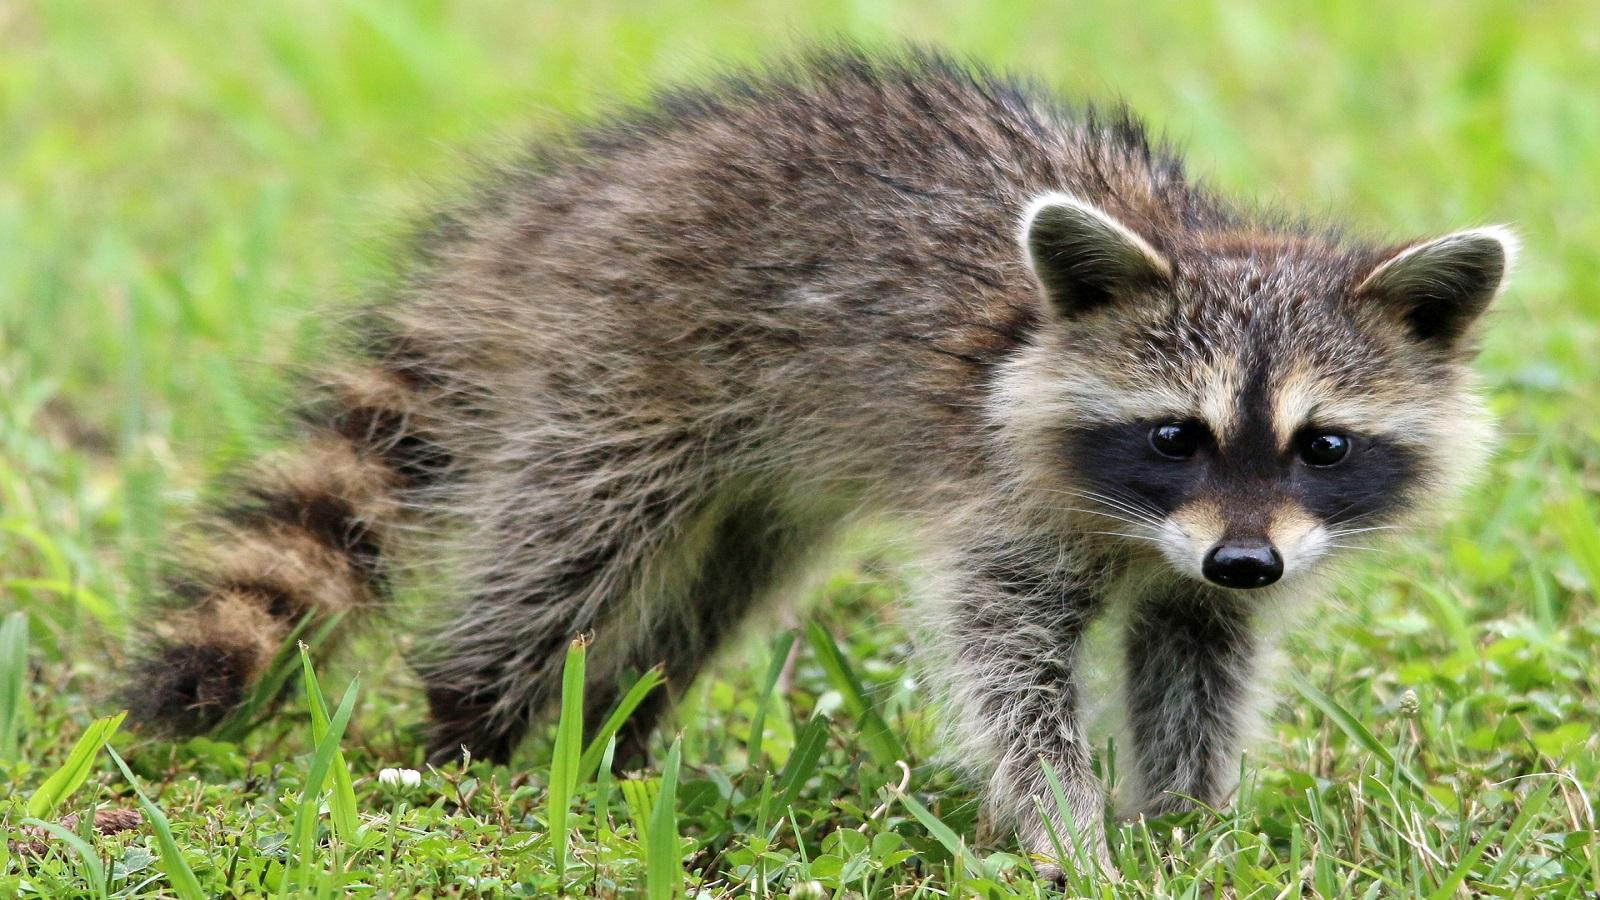
\includegraphics[width=0.666\textwidth]{Alle/Bild.jpg} \par BILDBESCHREIBUNG
			}\\
		 \hline
		  \multicolumn{2}{l}{\large{ \textbf{}}}\\
		 \hline
		  \bfseries{\small{Participation in competitions,\par Awards}} & \small{/}\\
		 \hline 
		  \multicolumn{2}{l}{\large{ \textbf{}}}\\
		 \hline
		  \bfseries{\small{Accesibility
			of\par Diploma Thesis}} & \small{Department administration}\\ 
		 \hline 
		  \multicolumn{2}{l}{\large{ \textbf{}}}\\
		\end{tabular}  
		
		\begin{tabular} {|p {5.7cm}|p{5.3cm}|p{4.6cm}|}
		 \hline
	   \vspace{5mm}
		  \bfseries{\small{Approval\par (Date/Signature)}} \vspace{5mm} & \tiny{Examiner} & \tiny{Head of College/Department}\\ 
		 \hline 
		\end{tabular} 
		\end{centering}

\thispagestyle{empty}


\newpage 
	\thispagestyle{empty}
	
	\begin {center}
	\begin{tabular} {|p {3cm}|p{8cm}|p{4.55cm}|}
	 \hline 
	\vspace{1mm}
	 \centering{
\includegraphics[width=0.20\textwidth,page=1]{Alle/TGM_logo.pdf}} &
	\centering{\normalsize{\textbf{HTBLVA Wien 20}}\par\small{\textbf{H�here Technische Lehranstalt f�r}\par Biomedizin- und Gesundheitstechnik}} &
		\small{\bfseries{Reife- und\par Diplompr�fung}}\\ 
		\hline
	\end{tabular}
	
	\vspace{5mm}
	\Large{\textbf{DIPLOMARBEIT\\}}
	\vspace{1mm}
	\small{\textbf{DOKUMENTATION\\}}
	\vspace{5mm}  
	
		\begin{tabular} {|p {5.7cm}|p{10.3cm}|}
		 \hline 
			\bfseries{\small{Namen der\par Verfasser/innen}} & \small{Fatiha Banata, Claudia Fuchs, Julia Gartner, Sumaiya Hossain}\\
		 \hline
		  \bfseries{\small{Jahrgang\par Schuljahr}} & \small{5AHBG 2022/23}\\
		 \hline 
		  \bfseries{\small{Thema der Diplomarbeit}} & \small{Sleep-Analyzer}\\ 
		 \hline 
		  \bfseries{\small{Kooperationspartner}} & \small{/}\\ 
		 \hline
		\multicolumn{2}{l}{\large{ \textbf{}}}\\
		 \hline
		  \bfseries{\small{Aufgabenstellung}} & \small{Im Rahmen einer Machbarkeitsstudie soll der Schlaf eines Anwenders durch Messung von Biosignalen analysiert werden. Dazu sollen verschiedene Messmethoden entwickelt und auf ihre Tauglichkeit getestet werden. Die gemessenen Daten sollen anschlie�end in einer Datenbank verwaltet und f"ur den Anwender in einer App dargestellt werden.}\\
		 \hline
		\multicolumn{2}{l}{\large{ \textbf{}}}\\ 
		 \hline
		  \bfseries{\small{Realisierung}} & \small{Die REM-Schlafphase wird mittels Elektrookulogramm zur Messung von Augenbewegungen detektiert und die vom ESP8266 gemessenen Daten werden "uber WLAN an eine Datenbank weitergegeben. Die Ausgabe der Daten erfolgt "uber ein App-Interface. }\\   
		 \hline
		\multicolumn{2}{l}{\large{ \textbf{}}}\\ 
		 \hline
		  \bfseries{\small{Ergebnisse}} & \small{Augenbewegungen lassen sich mittels EOG-Schaltung messen und die Daten, durch ein RTC-Modul mit einem Zeitstempel versehen, an die Datenbank schicken. In der App k"onnen die Daten f"ur den Anwender angezeigt werden.}\\
		 \hline
		\end{tabular}
	\end {center}
\thispagestyle{empty}
		
\newpage
\thispagestyle{empty}

	\begin{centering}
	\begin{tabular} {|p {3cm}|p{8cm}|p{4.55cm}|}
	 \hline 
	\vspace{1mm}
	 \centering{
\includegraphics[width=0.20\textwidth,page=1]{Alle/TGM_logo.pdf}} &
	\centering{\normalsize{\textbf{HTBLVA Wien 20}}\par\small{\textbf{H�here Technische Lehranstalt f�r}\par Biomedizin- und Gesundheitstechnik}} &
		\small{\bfseries{Reife- und\par Diplompr�fung}}\\ 
		\hline
		\multicolumn{3}{l}{\large{ \textbf{}}}\\
	\end{tabular} 
	
   \vspace {1mm}
	
		\begin{tabular} {|p {5.7cm}|p{10.3cm}|}
		 \hline 
			\bfseries{\small{Typische Grafik, Foto etc.\par (mit Erl�uterung)}} & \vspace{0.0mm} \small{
			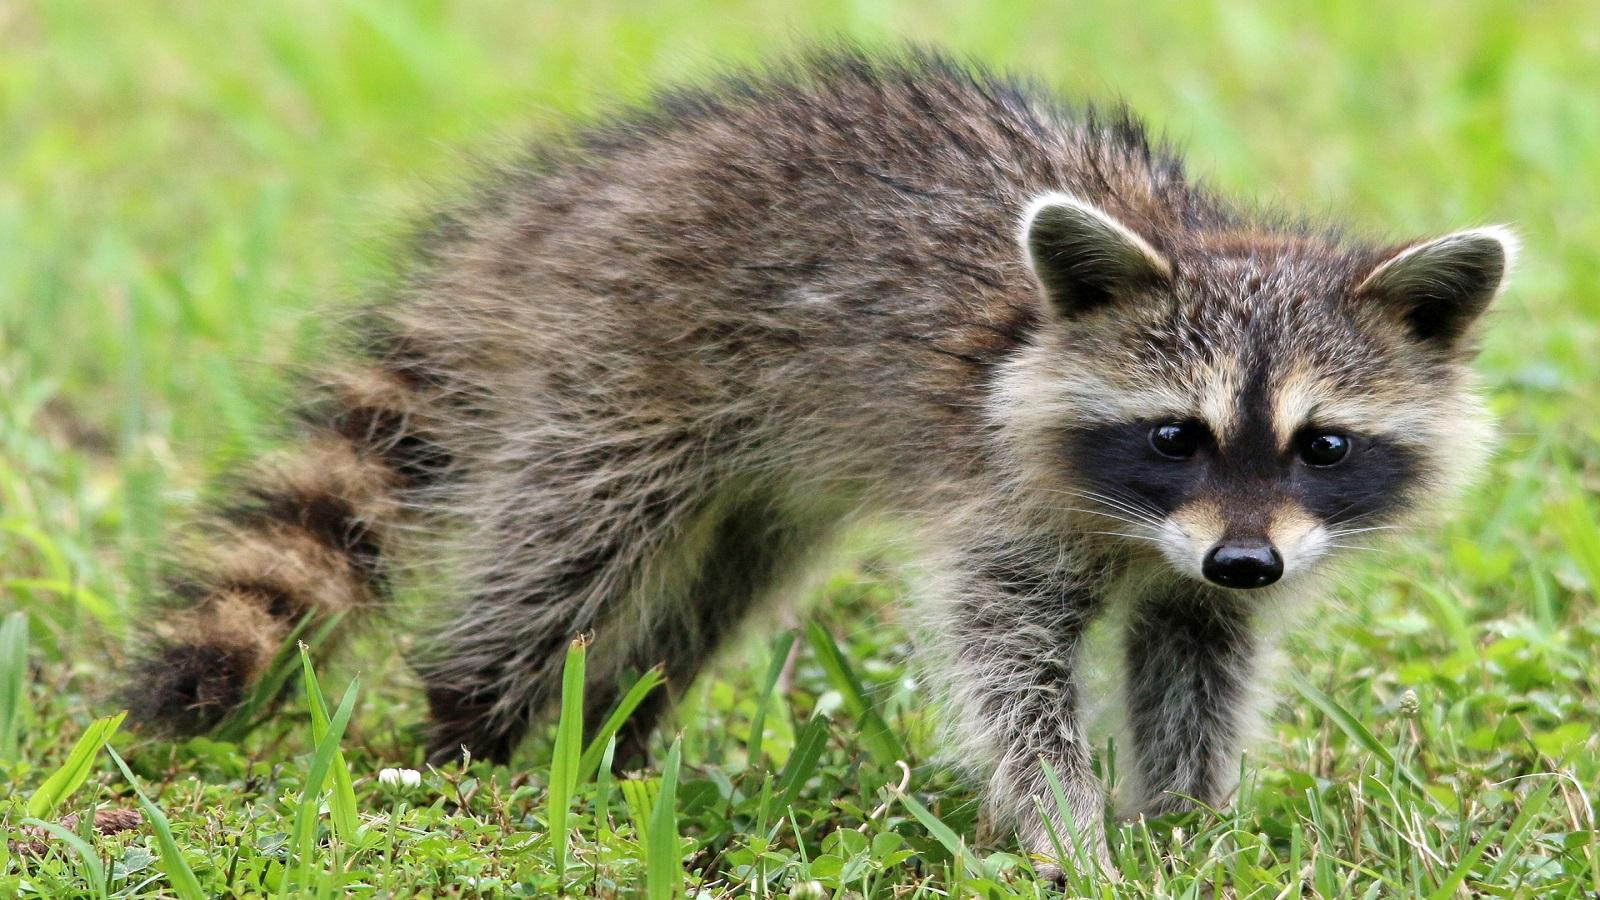
\includegraphics[width=0.666\textwidth]{Alle/Bild.jpg} \par BILDBESCHREIBUNG
			}\\
		 \hline
		  \multicolumn{2}{l}{\large{ \textbf{}}}\\
		 \hline
		  \bfseries{\small{Teilnahme an Wettbewerben,\par Auszeichnungen}} & \small{/}\\
		 \hline 
		  \multicolumn{2}{l}{\large{ \textbf{}}}\\
		 \hline
		  \bfseries{\small{M�glichkeiten der\par Einsichtnahme in die Arbeit}} & \small{Abteilungsadministration}\\ 
		 \hline 
		  \multicolumn{2}{l}{\large{ \textbf{}}}\\
		\end{tabular} %done 
		
		\begin{tabular} {|p {5.7cm}|p{5.3cm}|p{4.6cm}|}
		 \hline
	   \vspace{5mm}
		  \bfseries{\small{Approbation\par (Datum/Unterschrift)}} \vspace{5mm} & \tiny{Pr�fer/Pr�fernin} & \tiny{Direktor/Direktorin\par Abteilungsvorstand/Abteilungsvorst�ndin}\\ 
		 \hline 
		\end{tabular} 
		\end{centering}
		
\thispagestyle{empty}



\newpage
\fancyfoot[RE,LO]{Autor: Fatiha Bananta, Claudia Fuchs, Julia Gartner, Sumaiya Hossain}

\section{Einleitung}\label{einleitung}

Hier steht die Einleitung

\fancyfoot[RE,LO]{Autor: Fatiha Banata, Claudia Fuchs, Julia Gartner, Sumaiya Hossain}

\section {Schlaf} \label {schlaf}



%DIPLOMARBEIT
\newpage
\fancyfoot[RE,LO]{Autor: Claudia Fuchs}

\section {EOG} \label {eog}

\subsection {Einleitung} \label {eog einleitung}

Die Elektrookulografie ist ein Messverfahren, womit Augenbewegungen gemessen werden k"onnen. Die Messung basiert dabei auf der Potentialdifferenz zwischen der vorne gelegenen, positiv geladenen Cornea (Hornhaut) und der hinten gelegenen negativ geladenen Retina (Netzhaut). Das Auge kann also als Dipol betrachtet werden, dessen Spannung sich bei Bewegungen des Auges ver"andert. Diese Ver"anderung kann mittels Oberfl"achenelektroden in Augenn"ahe gemessen und in einem Elektrookulogramm dargestellt werden. \cite{reg205}

\begin{figure}[h]
	\centering
		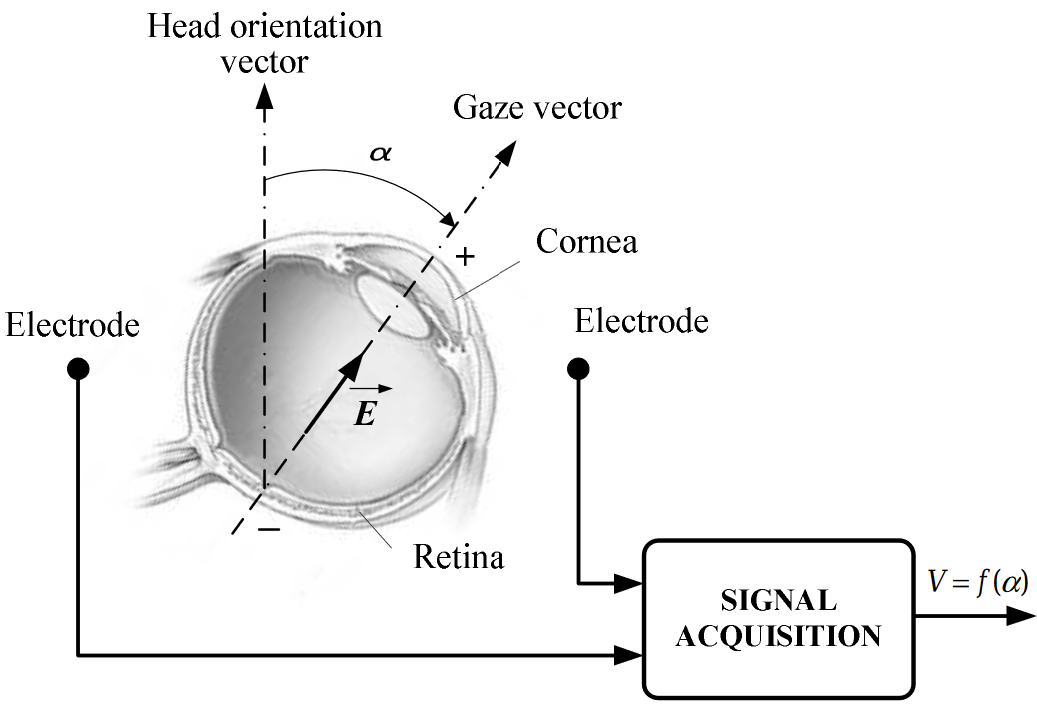
\includegraphics[width=0.9\textwidth]{Fuchs/Augendipol.png}
	\caption{Veranschaulichung des Augendipols durch Potentialdifferenz von Retina und Cornea}
	\label{fig:Augendipol}
\end{figure}

Abbildung \ref{fig:Augendipol} bildet den Blickvektor sowie dessen Ver"anderungspotential ab.  Eine Augenbewegung um $\alpha$ kann "uber die Elektroden gemessen und das Signal durch eine entsprechende Messschaltung aufbereitet werden. \cite{reg205}\\
Im Rahmen unseres Diplomprojekts soll es aber vorallem um die Schlafanalyse gehen. Wie bereits im Kapitel \ref{schlaf} er"ortert, zeichnet sich die REM-Schlafphase durch schnelle Augenbewegungen aus. Diese gilt es mittels EOG-Schaltung als solche zu erkennen. 

\subsubsection {Signalparameter} \label {signalparamater}

Bevor eine Messschaltung entwickelt werden kann ist es wichtig, die Signalparamter wie Amplitude und Bandbreite des zu messenden Biosignals in Erfahrung zu bringen.\\
Im Falle des EOGs ist die Amplitude typischerweise zwischen 0.05 und 3.5mV je nach Umgebung, Elektrodenplatzierung und St"arke der Augenbewegung. Die Bandbreite reicht von 0 bis 50Hz, wobei die meiste Information des Signals zwischen 0.1 und zirka 40Hz steckt. \cite{reg205},\cite{reg203}

INA-Testmessung
\subsubsection {Elektroden} \label {elektroden} 
Es gibt mehrere M"oglichkeiten, die Elektroden zur EOG-Messung im Gesicht anzubringen. Diese Unterscheiden sich sowohl in Position und Anzahl der Elektroden sowie der daraus resultierenden Genauigkeit der Messung.
\begin{figure}[h]
	\centering
		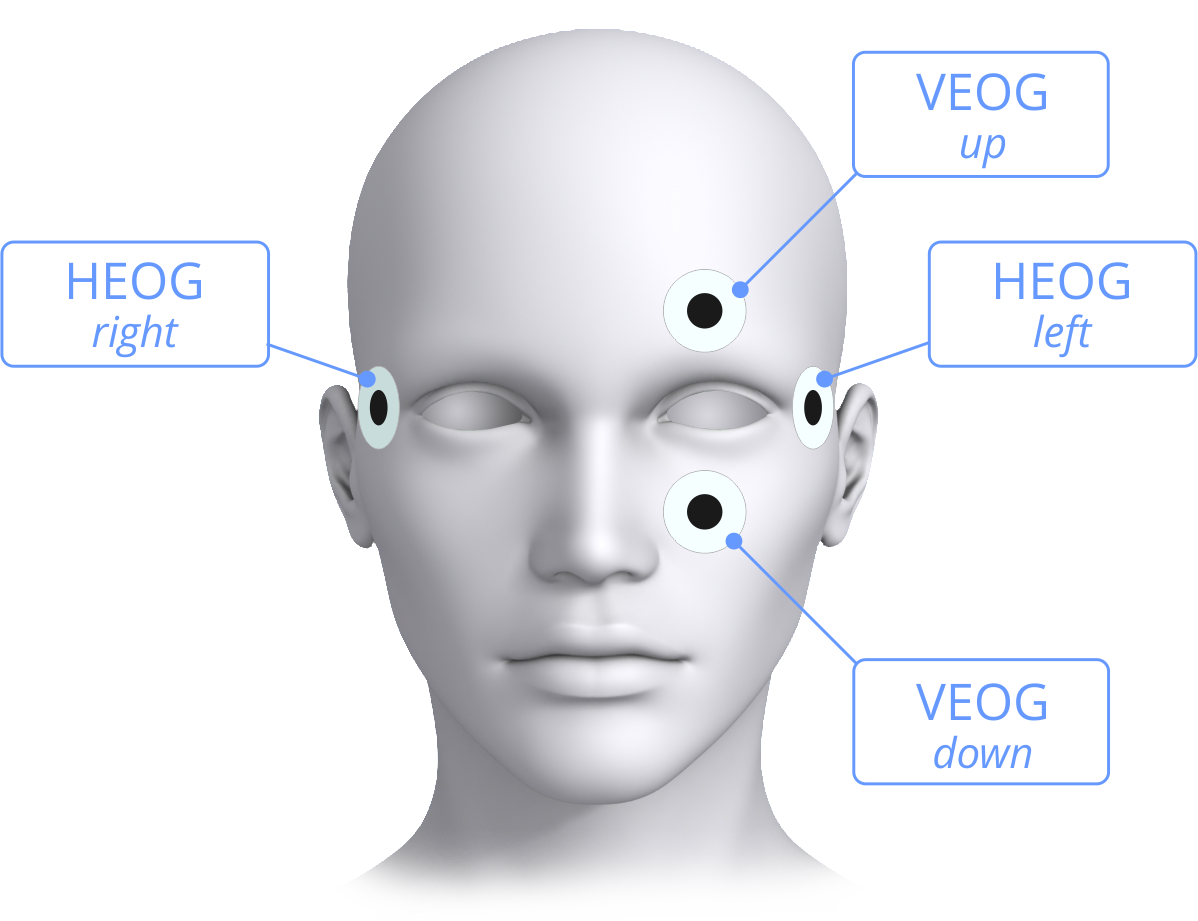
\includegraphics[width=0.9\textwidth]{Fuchs/Elektrodenplatzierung.png}
	\caption{Elektrodenplatzierung zur Messung horizontaler und vertikaler Augenbewegungen}
	\label{fig:Elektrodenplatzierung}
\end{figure}
F"ur unser Diplomprojekt wurde eine Methode mit 4 Elektroden gew"ahlt, welche in Abbildung \ref{fig:Elektrodenplatzierung} dargestellt wird. Zur Messung der vertikalen Augenbewegungen dienen dazu die "uber und unter dem Augen liegenden Elektroden, die Messung der horizontalen Augenbewegung erfolgt "uber die links und rechts angebrachten Elektroden. \\
Es handelt sich hierbei um Ag/AgCl-Oberfl"achenelektroden, welche auch bei EKG-Messungen verwendet werden k"onnen. 
\subsection {Signalflussdiagramm} \label {signalfluss}
\begin{figure}[H]
	\centering
		
\includegraphics[width=0.9\textwidth]{Fuchs/Signalfluss.png}
	\caption{Signalflussdiagramm des EOGs.}
	\label{fig:signalfluss}
\end{figure}

In Abbildung \ref{fig:signalfluss} werden die einzelnen Bestandteile, die fu"r die Messung der Augenbewegungen ben"otigt werden, in einem Signalflussdiagramm dargestellt. Der genaue Aufbau dieser und die Dimensionierung der dazugeh"origen Bauteile werden in den n"achsten Abschnitten erl"autert. Es ist zus"atzlich anzumerken, dass es sich hierbei lediglich um die Messschaltung von einer Richtung (vertikal oder horizontal) handelt. Die Gesamtschaltung besteht demnach aus zwei identen Schaltungen, die sich einen ADC und Mikrocontroller teilen. 

\subsection {Filter} \label {filter}
Wie bereits im Kapitel \ref{signalparamater} erw"ahnt, betr"agt die f"ur uns relevante Bandbreite 0.1-40Hz. Wir ben"otigen also einen Hochpass, um die Gleichspannungskomponenten herauszufiltern und einen Tiefpass, der Frequenzen "uber 50Hz d"ampft und zugleich als Anti-Aliasingfilter f"ur den Analog-Digital-Wandler dient.\\
Es wurden dazu aktive Filter des Sallen-Key-Typs ausgew"ahlt und dimensioniert.

\subsubsection {Hochpass (2. Ordnung)} \label{hp}
\begin{figure}[H]
	\centering
		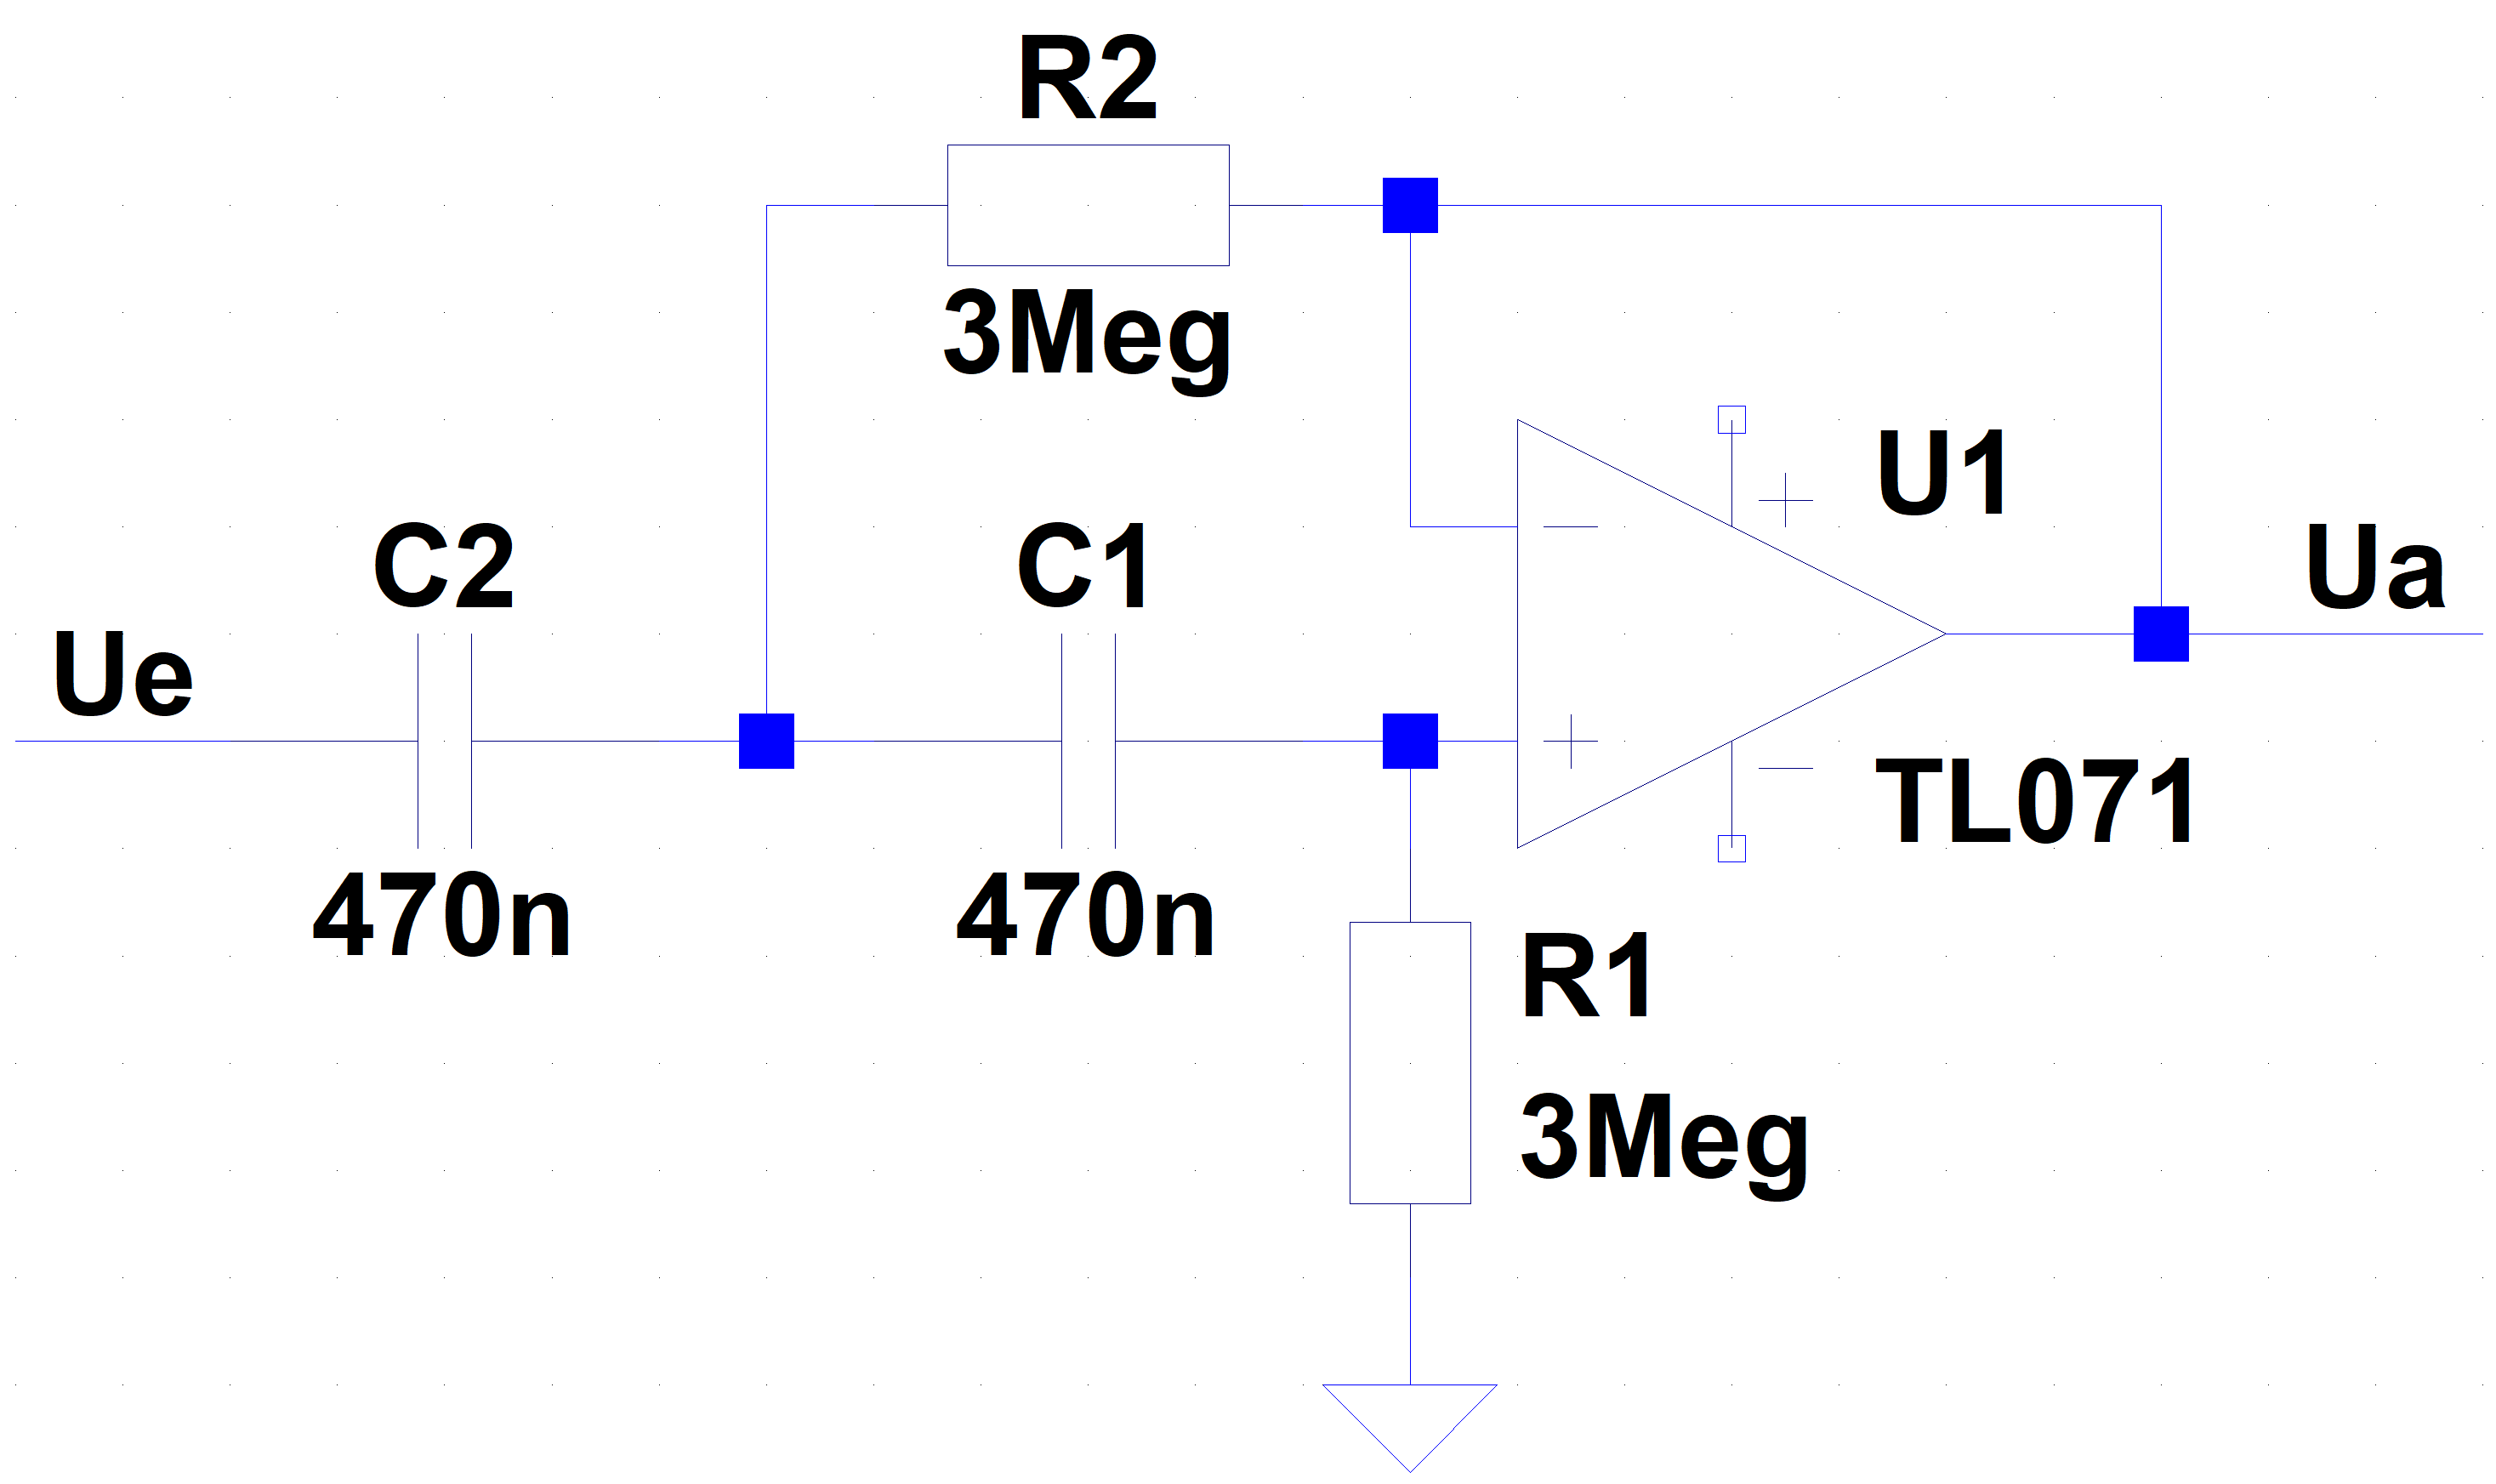
\includegraphics[width=0.9\textwidth]{Fuchs/Hochpass.png}
	\caption{OPV-Schaltung eines Hochpasses 2.Ordnung}
	\label{fig:hp}
\end{figure}

Zur Filterung des Gleichspannungsanteils wurde eine Schaltung, wie in Abbildung \ref{fig:hp} gezeigt, dimensioniert. Es handelt sich dabei um einen Hochpass zweiter Ordnung mit einer Grenzfrequenz $f_g = 0.11Hz$.

\subsubsection {Anti-Aliasing-/Tiefpassfilter (3.Ordnung)} \label{tp}
\begin{figure}[H]
	\centering
		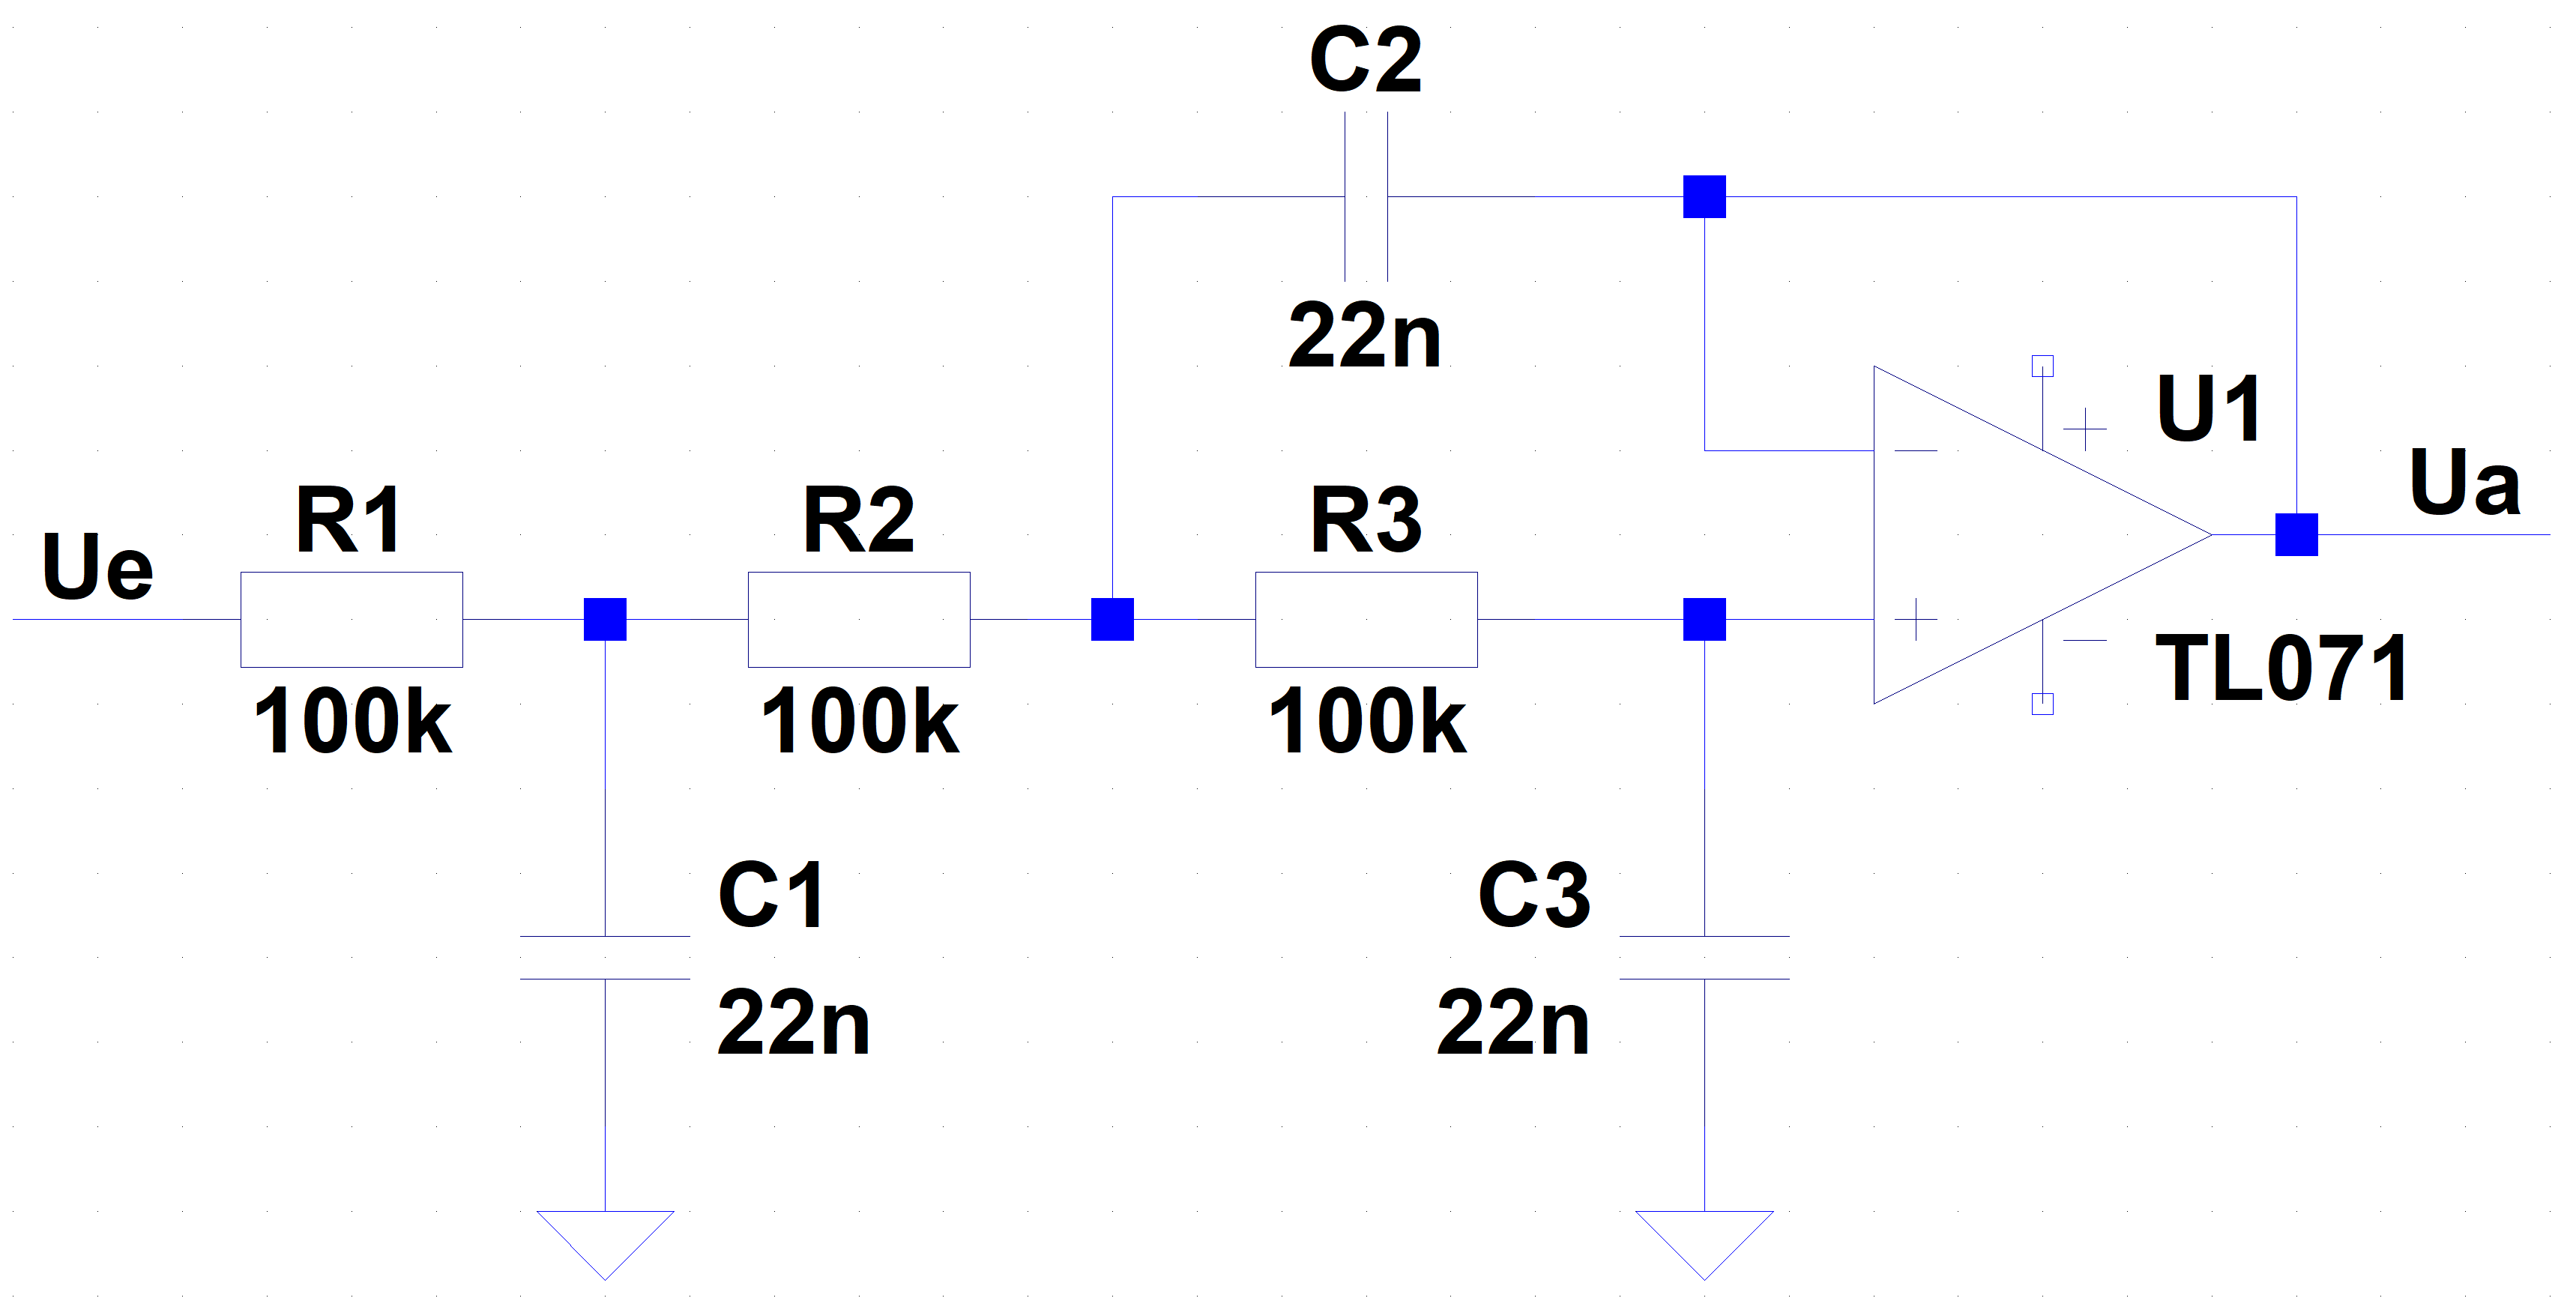
\includegraphics[width=0.9\textwidth]{Fuchs/Tiefpass.png}
	\caption{OPV-Schaltung eines Tiefpasses 3.Ordnung}
	\label{fig:tp}
\end{figure}

Zur D"ampfung h"oherer Frequenzen, die nicht zu unserem Nutzsignal geh"oren, wurde ein Tiefpass 3.Ordnung, wie in Abbildung \ref{fig:tp} gezeigt, dimensioniert. Die Grenzfrequenz betr"agt $f_g = 72Hz$\footnote{Die Bandbreite des Nutzsignals endet bereits bei ~40Hz. Die h"oher gew"ahlte Grenzfrequenz ist mit der Ordnung des Filters begr"undet, bei dessen Grenzfrequenz bereit -12dB des Signals ged"ampft werden, die eigentliche Grenzfrequenz (bei einer D"ampfung von -3dB) liegt also tiefer.}.

Welche Art von Filter, Bauteilwerte

\subsection {Verst"arkung} \label {verstaerkung}

Wie bereits im Kapitel \ref{signalparamater} erw"ahnt, handelt es sich beim EOG-Signal, wie bei den meisten Biosignalen, um eher kleinere Amplituden (0.05-3.5mV). Diese gilt es erst einmal messtechnisch zu verst"arken, um brauchbare Ergebnisse zu erhalten.

\subsubsection {Instrumentenverst"arker} \label{ina}
Der Instrumentenverst"arker verst"arkt die Differenz zwischen den beiden Eingangsspannungen. In unserem Fall die Differenz zwischen zwei Elektroden ("uber/unter dem Auge bzw. links und rechts der Augen). Die Verst"arkungsformel zur Dimensionierung f"ur den INA128 kann aus dem Datenblatt abgelesen werden und lautet:\\
\begin{equation}\label{eq:ina}
	G = 1 + {50k\Omega}/{R_G}
\end{equation}

Der Einfachkeit halber wurde $R_G$ zun"achst mit $1k\Omega$ angenommen. Daraus ergibt sich eine Verst"arkung von 51.

\paragraph {Testmessung der Rohdaten} \label {Rohdaten}
\textbf{\\Messschatltung:}
\begin{figure}[H]
	\centering
		
\includegraphics[width=0.9\textwidth]{Fuchs/Messschaltung-Rohdaten.png}
	\caption{Schaltung zur Messung der Rohdaten}
	\label{fig:ms_rohdaten}
\end{figure}

Der Verst"arkungswiderstand $R_G$ der in Abbildung \ref{fig:ms_rohdaten} dargestellt ist, entspricht $1k\Omega$ wie bei Gleichung \ref{eq:ina} berechnet. Die Versorgungsspannung mit $\pm5V$ sowie das Oszilloskop selbst sind Funktionen des AnalogDiscovery, einem portablen Oszilloskop, welche in Kapitel \ref{analogdiscovery} n"aher beschrieben werden. \\

\textbf{Messergebnisse:}
\begin{figure}[H]
	\centering
		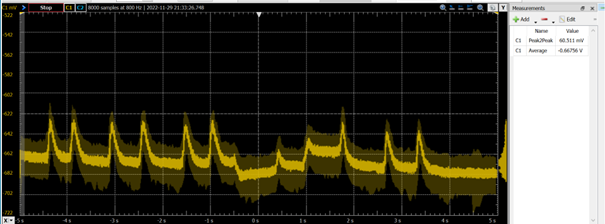
\includegraphics[width=0.9\textwidth]{Fuchs/Messergebnis_RohdatenV.png}
	\caption{Messung der Rohdaten von Augenbewegungen in vertikaler Richtung}
	\label{fig:me_rohdatenV}
\end{figure}
\begin{figure}[H]
	\centering
		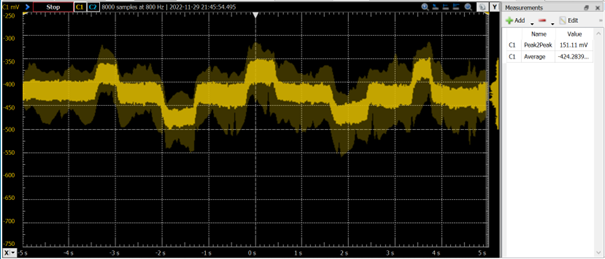
\includegraphics[width=0.9\textwidth]{Fuchs/Messergebnis_RohdatenH.png}
	\caption{Messung der Rohdaten von Augenbewegungen in horizontaler Richtung}
	\label{fig:me_rohdatenH}
\end{figure}

Die zwei obenstehenden Abbildungen \ref{fig:me_rohdatenH} zeigen die Messungen der Rohdaten mit einer Verst"arkung von 51. Bei der Messung der Augenbewegungen in vertikaler Richtung, wie in Abbildung \ref{fig:me_rohdatenV} dargestellt, ist das Blinzeln, welche sich durch steile Amplitudenanstiege kennzeichnet, deutlich zu erkennen. Die maximale Amplitude betr"agt ca. $40-60 mV$. Dividiert man das durch die Verst"arkung, ergibt sich ein Amplitudenwert von $80-110\mu V$. Auff"allig ist der negative Offset von rund $0.667V$.

Invertierender/nicht invertierender

\subsection {AD-Wandlung} \label {adc}

allgemeines

\subsubsection {MCP3208} \label {mcp3208}

Bauteilbeschreibung, Datenblatt!

\subsubsection {Offset} \label{offset}



\subsection {ESP8266} \label {esp}

\textbf{\\Pinout:\\} 
\begin{figure}[h]
	\centering
		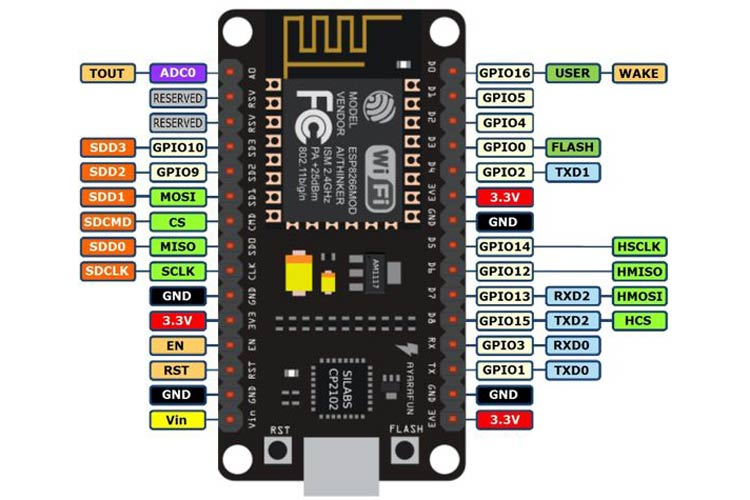
\includegraphics[width=0.9\textwidth]{Alle/ESP8266_Pinout.jpg}
	\caption{Pinout des ESP8266 NodeMCUs}
	\label{fig:esp_pinout}
\end{figure}

Funktionen, Abtastung

\subsection {Analog Discovery} \label{analogdiscovery}

\subsection {Schnittstellen} \label {schnittstellen}

\subsubsection {SPI} \label {spi}

SPI-Schnittstelle allgemein
Pinbelegung, Kommunikation

\subsubsection {Serielle Schnittstelle} \label {serial}

\paragraph {Matlab} \label{matlab}

\subsection {Messergebnisse} \label {messergebnis}





\newpage
\fancyfoot[RE,LO]{Autor: Julia Gartner}

\section {Mobile Applications} \label {MobileApplications}

\subsection {Einleitung} \label {MAEinleitung}

Eine Mobile Application, oft nur App genannt, ist Software, die auf mobilen Ger�ten verwendet werden kann. Solche Ger�te sind z.B. Smartphones, Tablets oder Smartwatches und haben meistens entweder Android oder iOS als Betriebssystem\cite{reg401}. Generell gibt es viele Anwendungen f�r mobile App wie Kommunikation, E-Commerce und Weiterbildung\cite{reg402}. In unserem Fall hat das Software Interface prim�r die Aufgabe, die mithilfe des EOGs gesammelten Daten f�r den User graphisch darzustellen. Sekund�r gibt es eine Weckerfunktion.

\subsection {Allgemeines zur Mobilapp-Entwicklung} \label {MAAllgemeines}

Wie bereits in Kapitel \ref{MAEinleitung} erw�hnt, sind die meistverbreiteten Betriebssysteme, die die Umgebung f�r Mobile Apps darstellen, iOS und Android mit einem Marktanteil von 99\% im Jahr 2018 in den USA. Mobile Apps f�r diese beiden Betriebssysteme werden jedoch nicht in der selben Sprache geschrieben. F�r Android kann in Java oder Kotlin geschrieben werden, w�hrend f�r iOS Objective-C oder Swift verwendet wird. Das ist in der Praxis oft nicht optimal, da eine Anwendung erstens in zwei verschiedenen Sprachen geschrieben werden muss und zweitens auch zwei verschiedene Anwendungen gewartet werden m�ssen\cite{reg403}. Eine L�sung f�r dieses Problem sind Hybrid Mobile App Development Frameworks. Mit diesen Frameworks k�nnen Apps in einer Sprache geschrieben werden und trotzdem auf verschiedenen Betriebssystemen laufen\cite{reg404}.\\

\begin{figure}[H]
	\centering
		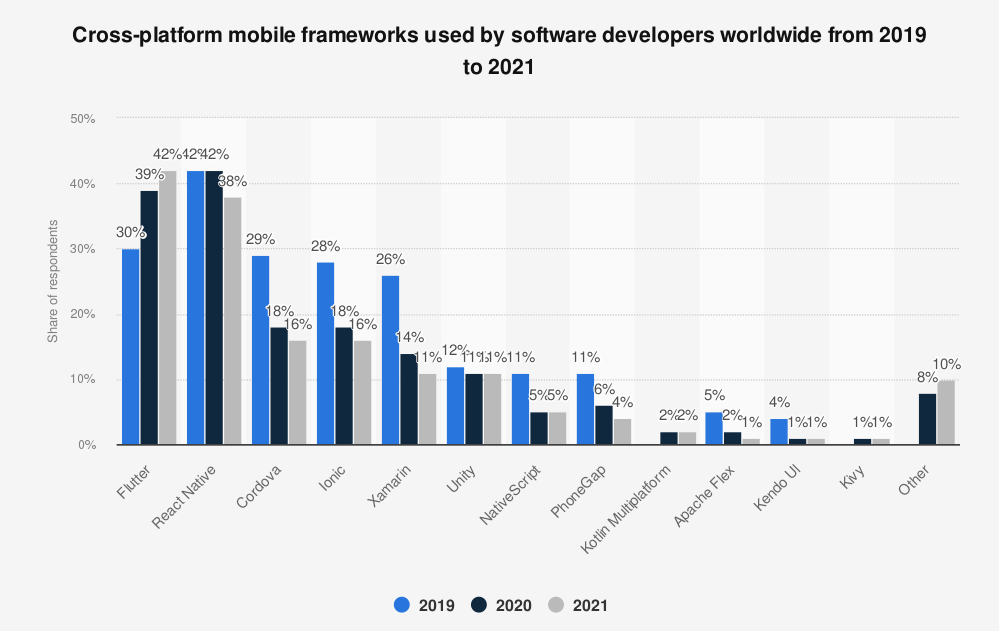
\includegraphics[width=0.9\textwidth]{Gartner/assets/cross_platform_use_statistic.png}
	\caption{Plattform�bergreifende Mobile-Frameworks die von Softwareentwicklern weltweit verwendet werden (2019 bis 2021)\cite{reg405}}
	\label{fig:cross_platform_use_statistic}
\end{figure}

Wie in Abbildung \ref{fig:cross_platform_use_statistic} zu sehen ist, sind die zwei meist verwendeten plattform�bergreifenden Mobile-Frameworks seit 2019 Flutter und React Native, was sich immer weiter absetzt. W�hrend im Jahr 2019 das meistverwendete Framwork noch React Native war, verwenden 2021 die meisten Entwickler bereits Flutter.  \\
React Native und Flutter unterscheiden sich in mehreren Hinsichten. Zum einen wird das React Native-Framework mit JavaScript verwendet, w�hrend ein Flutter-Projekt in Dart geschrieben wird. React Native erreicht die plattformunabh�ngige Anwendung durch eine Br�cke; ein React Native-Projekt in JavaScript auf einem Android-Ger�t z.B. kommuniziert �ber diese Br�cke mit nativen Komponenten des Betriebssystems. Bei Flutter hingegen wird ein Projekt beim Kompilieren von Dart direkt zu einer nativen Sprache �bersetzt, f�r ein Ger�t ist das also nicht zu unterscheiden von einer nativen App\cite{reg406}.

\subsubsection {Entwicklungsumgebung} \label{MAEntwicklungsemgebung}

VSCode, Android Studio Emulator

\subsection {Flussdiagramm} \label {MAFlussdiagramm}

\begin{figure}[H]
	\centering
		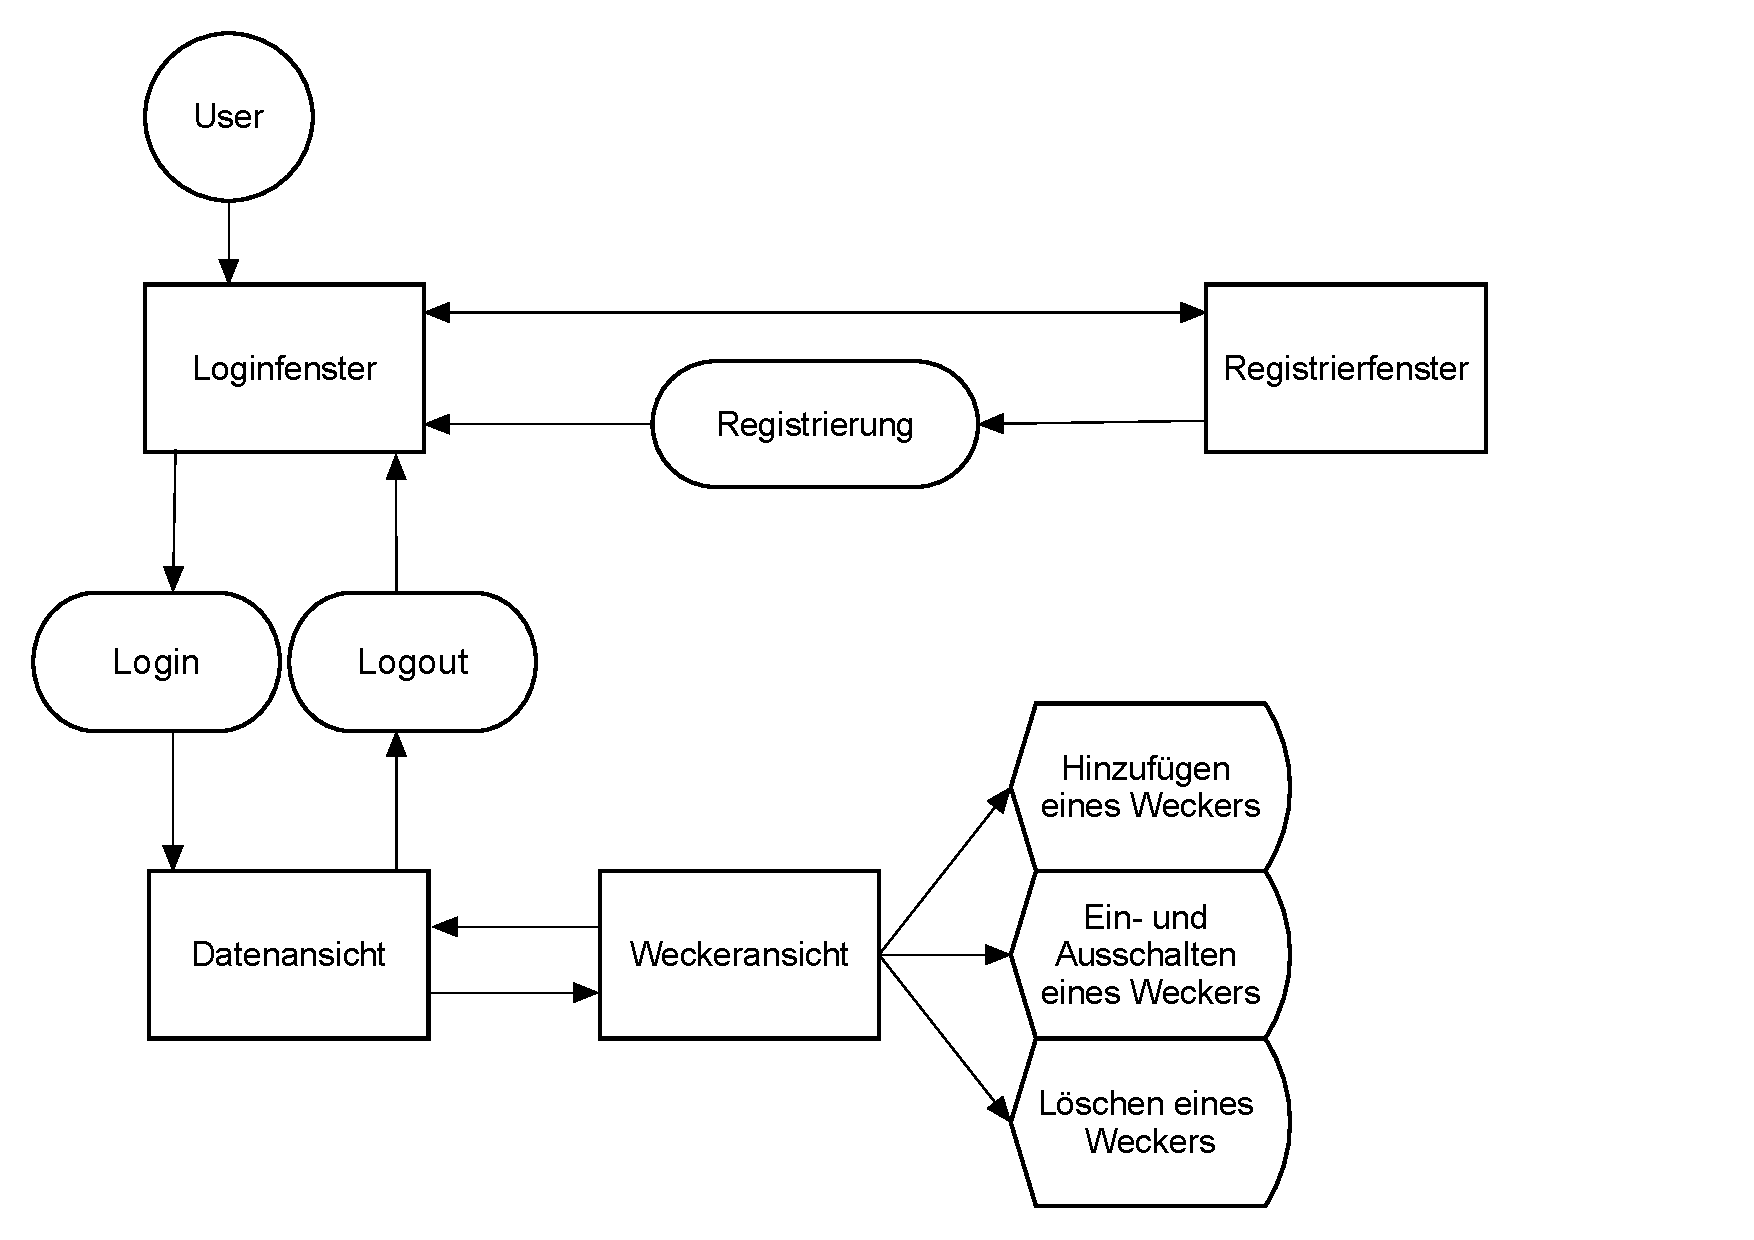
\includegraphics[width=0.9\textwidth]{Gartner/flussdiagramm.pdf}
	\caption{Flussdiagramm der Mobile Application}
	\label{fig:MA_Flussdiagramm}
\end{figure}

\begin{figure}[H]
	\centering
		
\includegraphics[width=0.45\textwidth]{Gartner/buffer.jpg}
	\caption{Loginfenster des GUI}
	\label{fig:MA_Loginfenster}
\end{figure}

\begin{figure}[H]
	\centering
		
\includegraphics[width=0.45\textwidth]{Gartner/buffer.jpg}
	\caption{Registrierfenster des GUI}
	\label{fig:MA_Registrierfenster}
\end{figure}

Der erste Bildschirm ist wie in Abbildung \ref{fig:MA_Flussdiagramm} zu erkennen entweder das Loginfenster oder der Homescreen mit der Datenansicht. Falls man die App zum ersten Mal �ffnet oder sich in der letzten Session abgemeldet hat, ist das in Abbildung \ref{fig:MA_Loginfenster} zu sehende Loginfenster der Startpunkt. Von hier aus kann sich der Benutzer entweder einloggen, wenn er schon einen Account hat, oder zum Registrierfenster, wie in Abbildung \ref{MA_Registrierfenster} gezeigt, wechseln, um sich zu registrieren. Wenn die Registrierung erfolgreich war, wird wieder zum Loginfenster geleitet. Es gibt aber auch die M�glichkeit, ohne Registrierung wieder zum Loginfenster zu wechseln. In beiden F�llen muss der Login im Loginfenster erfolgen, um die Datenansicht zu laden. \\

\begin{figure}[H]
	\centering
		
\includegraphics[width=0.45\textwidth]{Gartner/buffer.jpg}
	\caption{Datenansicht des GUI}
	\label{fig:MA_Datenansicht}
\end{figure}

Im Fall, dass der User sich bereits einmal eingeloggt und in der letzten Session nicht abgemeldet hat, wird direkt die Datenansicht geladen. Hier gibt es, wie in Abbildung \ref{MA_Datenansicht} zu sehen, eine Navigationsleiste am unteren Ende des Bildschirms, mit dem ausgew�hlt werden kann, ob die Daten- oder Weckeransicht gezeigt wird. \\
In der Datenansicht werden alle Messergebnisse der EOG-Messungen eines Benutzers angezeigt. Hier gibt es, abgesehen vom Scrollfeature, keine Interaktionsm�glichkeiten. \\

\begin{figure}[H]
	\centering
		
\includegraphics[width=0.45\textwidth]{Gartner/buffer.jpg}
	\caption{Weckeransicht des GUI}
	\label{fig:MA_Weckeransicht}
\end{figure}

Die Weckeransicht, gezeigt in Abbildung \ref{fig:MA_Weckeransicht}, erm�glicht eine Verwaltung der Weckerfunktion. M�gliche Interaktionen hier sind das Hinzuf�gen oder Entfernen und das Ein- oder Ausschalten eines Weckers. Hinzugef�gte Wecker werden ebenfalls hier angezeigt. \\

\begin{figure}[H]
	\centering
		
\includegraphics[width=0.45\textwidth]{Gartner/buffer.jpg}
	\caption{Logout des GUI}
	\label{fig:MA_Logout}
\end{figure}

Wie bereits in Abbildung \ref{MA_Datenansicht} und \ref{MA_Weckeransicht} zu erkennen, ist links oben in der Ansicht ein Menu Button implementiert. Das dahinterliegende Menu mit der Logout-Funktion ist in Abbildung \ref{MA_Logout} zu sehen. 

\subsection {Funktionalit�t} \label {}

\subsubsection {Framework} \label {MAFramework} 

Wie bereits in Kapitel \ref{MAEinleitung}

\subsubsection {Benutzerverwaltung} \label {}

\subsubsection {State-Management} \label{MAState}

Es gibt zwei verschiedne Arten von Widgets in Flutter: Stateless und Stateful Widgets. Stateful Widgets sind Widgets, die sich ver�ndern k�nnen, wenn z.B. Daten dargestellt werden oder der Benutzer mit dem Widget interagieren kann. Stateless Widgets hingegen sind Widgets, die sich nie ver�ndern\cite{reg407}.\\
State ist Information, die ermittelt werden kann, w�hrend ein Widget gebaut wird und sich auch �ndern kann. Beim Entwickeln einer App in Flutter muss also darauf geachtet werden, dass beim Auftreten solcher �nderungen ein Widget auch neu aufgebaut wird, da die dahinterliegenden Informationen sich sonst ge�ndert haben, aber nicht das Widget selbst. Das kann mit Methoden wie z.B. setState geregelt werden\cite{reg408}. Hier k�nnen aber Probleme entstehen, wenn State �ber verschiedene Klassen hinweg weitergegeben werden muss; Dies kann zwar mit �bergabeparametern gel�st werden, aber auch hier bleibt das genannte Problem bestehen und vor allem bei gr��eren Projekten ist die L�sung bei weitem nicht ideal.\\
Im Internet k�nnen viele Klassen gefunden werden, die State Management vereinfachen sollen. Eine der Basisklassen ist die InheritedWidget class. Die Logik hinter der Klasse ist, dass State im Baum nach unten vererbt werden kann, sich die verkn�pften Widgets sich bei einer �nderung des States in einem dar�berliegenden Widget also auch neu aufbauen\cite{reg409}. 
F�r das Projekt Sleepanalyzer wurde die Klasse provider zusammen mit ChangeNotifier verwendet, was einer der popul�rsten Ans�tze ist. Klassen k�nnen als ChangeNotifier Klasse angelegt werden. Andere Klassen k�nnen dann subscriben, um bei �nderungen verst�ndigt zu werden. Die Klasse Provider sorgt daf�r, dass State nicht durch den ganzen Widgetbaum weitergegeben werden muss, sondern direkt zu einem bestimmten Widget weitergegeben werde kann. Dazu muss allerdings eine Liste in einem Widget �ber einem Provider und dem Widget, in dem der State gebraucht wird angelegt sein\cite{410}.

\subsubsection {Permanenter Speicher} \label{}

\subsubsection {Data Fetching} \label{MADataFetching}

Da bei der Messung des EOGs die Daten direkt vom Mikrocontroller zu einem Server geschickt werden und dort auf einer Datenbank gespeichert werden, m�ssen diese zur Ansicht der Daten in der App zuerst vom Server angefragt werden. Wenn in der App zur Datenansicht gewechselt wird, entweder vom Loginfenster oder von der Weckeransicht, wird von einem Widget eine Funktion aufgerufen, in der ein Post-Request an den Server gestellt wird. Der body dieses Requests enth�lt die momentan g�ltige User-ID. Am Server werden alle Daten, die zu dieser ID vorhanden sind gesammelt und ebenfalls in einem Post-Request im JSON-Format zur�ckgesendet. Diese Daten werden dann in der App weiter verwertet. Im Folgenden werden alle einzelnen Schritte n�her erl�utert. 

\paragraph{Async functions} \label{MADataFetching_AsyncFunctions}

Da Vorg�nge wie das Warten auf eine Antwort des Servers nach dem Senden eines POST-Requests lange dauern, w�re es nicht gut, wenn alle anderen Vorg�nge w�hrenddessen blockiert sind. Deshalb gibt es Unterscheidungen zwischen synchronen und asynchronen Vorg�ngen. Bei synchronen Operationen wird ein Schritt nach dem anderen abgehandelt, w�hrend bei asynchronen Operationen w�hrenddessen andere Operationen durchgef�hrt werden k�nnen. Die Klasse, die f�r asynchrone Vorg�nge im Flutter-Framework verwendet wird ist die Future\flq T\frq{} Klasse. Ein \glqq future\grqq{} ist eine Instanz der Klasse Future und ist das Ergebniss einer asynchronen Funktion. Wenn nun eine asynchrone Funktion aufgerufen wird, wird ein unvollst�ndeiges future zur�ckgegeben. Dieses future wartet auf den wirklichen Wert, der von der Funktion zur�ckgegeben wird (falls eine Funktion einen R�ckgabewert hat). \\
Dies sorgt daf�r, dass w�hrend auf die Antwort des Servers gewartet werden muss, alle anderen Vorg�nge in der App weiter bestehen bleiben.

\paragraph{HTTP Requests} \label{}

Es gibt eine Reihe von Requests, die im HTTP-Protokoll angef�hrt sind und oft in zur Datenvermittelung verwendet werden. Zwei der h�ufigsten davon sind der POST- und der GET-Request. Diese beiden unterscheiden sich in mehreren Hinsichten. Wie der Name es annehmen l�sst ist ein GET-Request urspr�nglich f�r die Anfrage an einen Server nach Daten und ein POST-Request f�r das Vermitteln von Daten an den Server gedacht. Dies muss in der Praxis allerdings nicht immer eingehalten werden\cite{reg413}. \\
Einer der wichtigsten Unterschiede ist, dass bei einem GET-Request die gesamte Anfrage im Header eines Requests angef�hrt ist, und somit die L�nge auch an die maximale URL-L�nge eines Browsers angepasst werden muss; Ein GET-Request kann also f�r Internet Explorer zum Beispiel maximal 2.048 Zeichen, abz�glich der Anzahl der Zeichen des Pfads, betragen. \\
Bei einem POST-Request ist das nicht der Fall, da der Inhalt eines POST-Requests nicht im header, sondern im Message-body angef�hrt wird\cite{reg413},\cite{reg414}. \\

\paragraph {Implementierung} \label{MADataFetching_Implementierung}

\begin{figure}[H]
	\centering
		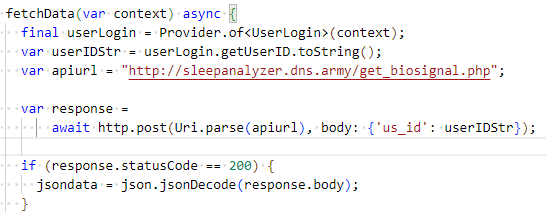
\includegraphics[width=0.9\textwidth]{Gartner/assets/async_post_json.png}
	\caption{Quellcodeausschnitt zur Kommunikation mit dem Server}
	\label{fig:async_post_json}
\end{figure}

In Abbildung \ref{fig:async_post_json} ist die Funktion zur Anfrage und Erhaltung der Daten vom Server zu sehen. Zuerst wird ein POST-Request geschickt, in dessen body die Benutzer-ID festgelegt ist. Die Antwort des Servers erfolgt im JSON-Format und muss dekodiert werden. 





\subsubsection {Graphische Darstellung der Daten} \label{}

syncfusion flutter charts

\subsubsection {Design} \label{}

Material Design








\newpage
\fancyfoot[RE,LO]{Autor: Sumaiya Hossain}

\section {Platine} \label {}

\subsection {RTC-Modul} \label {}

In diesem Kapitel wird das RTC Modul pr�sentiert, welches f�r das Projekt unverzichtbar ist. 

\subsubsection {Hintergrund} \label {}

Da der Benutzer eine bestimmte Uhrzeit einstellen kann f�r den Wecker, m�ssen mit den Messungen auch die Uhrzeit mitgegeben werden. Damit das m�glich ist wurde ein RTC-Modul gefertigt. 

\subsubsection {Bestandteile} \label {}

Die Schaltung des Real-Time-Clocks besteht aus einem Quarz, einer Knopfzellenbatterie und dem DS1302SN+. Das DS1302SN+ ist ein Trickle-Charge Timekeeping Chip, die auch ein Echtzeituhr und -kalender beinhaltet und sie sorgt daf�r, dass die App beim Auswerten der Messungen die genau Zeit kennt. Der Unterschied zum gew�hlten Chip und zum DS1302 ist, dass der gew�hlte eine andere Pin Package hat und die Temperatur Range geht von -40�C bis 85�C. Die Batterie dient dazu die Echtzeituhr am laufenden zu halten, wenn das RTC nicht versorgt wird.  

\subsubsection {Funktion} \label {}

Durch den Quarz wird eine Taktfrequenz erzeugt, welches erm�glicht, dass den Sekundentakt einer Uhr zu generieren.

\subsubsection {EOG-Platine} \label {}

Ein wichtiger Bestandteil dieses Projekts ist das EOG (siehe Kapitel Claudia), f�r die eine Platine angefertigt wurde. 
Die meisten SMD Bauteile waren verf�gbar sowohl in der Schule als auch in den Gesch�ften. Ein Problem gab es bei den 3M Ohm SMD Widerst�nde, die dann mit drei seriell geschalteten 1M Ohm SMD Widerst�nden ersetzt wurden. 
Die Platine wurde auf KiCad Version 6.0, ein Schaltplaneditor und Layoutprogram, angefertigt. Zuerst wurde eine Schematic erstellt, in der alle Bauteile verbunden wurden. Danach folgte die Footprint-Zuweisung der Bauteile. Ein Problem gab es bei dem ESP, denn eine passende Footprint war nicht vorhanden und musste daher erstellt werden. Anschlie�end konnte dann nach der Erstellung der PCB die eigentlichen Leiterbahnen f�r die Platinen nachgezogen werden. 


\newpage
\fancyfoot[RE,LO]{Autor: Fatiha Banata}

\section {Datenbank} \label {datenbank}

\subsection {Einleitung} \label { einleitung}

Der Sleep-Analyzer ist ein kompaktes Schlaflabor, das verschiedene Biosignale w�hrend des Schlafs misst und aufzeichnet. Die im Schlaf erfassten Messdaten werden in einer Datenbank gespeichert. Die vorliegenden Kapitel befassen sich zun\"achst mit der grundlegenenen Theorie eines Datenbankmanagementsystem. Anschlie�end werden die realisierten Schritte, die bei dem Entwurf der SleepAnalzer-Datenbank essentiell waren, erl\"autert. Des Weiteren widmet sich das Kapitel der Sicherheit von Daten. Abschlie�end wird die Konfiguration eines Servers veranschaulicht.


\subsection {Datenbankmanagementsystem} \label {datenbankmanagementsystem} 

Schnittstelle zwischen Datenbank und Anwender  

\subsection {MariadB} \label {mariadb}

Warum Mariadb? Unterschied zu anderen DBMS (MYSQL)

\subsection {Normalformen} \label {normalformen}

Was sind Normalformen, Funktionen 

\subsubsection {Erste Normalform} \label {erste normalform}

Alle Attributwerte m\"ussen atomar sein

\subsubsection {Zweite Normalform} \label {zweite normalform}

Alle Nichtschlu\"usselattribut voll funktional abh\"angig vom gesamten Prim\"arschl\"ussel

\subsubsection {Dritte Normalform} \label {dritte normalform}

Alle Nichtschl\"usselattribute sind voneinander unabh\"angig


\subsection {Entwicklung des Datenbanksytems} \label {entwicklung des datenbanksytem}

Zum Entwurf eines Datenbanksytem z\"ahlt die sowohl Anforderungsdefintion der Datenbank als auch die Defintion der Datentypen. Weiters wird mithilfe eines Entity-Realshionship-Modells (ER-Modell) eine Grunsdtruktur der Datenbak definiert. Hier werden die Entit\"aten und Beziehungen der einzelnen Tabellen konkretisiert.


\subsubsection {Anforderungsdefinition} \label {anforderungsdefinition}

Problembeschreibung, Anforderungen

\subsubsection {Entity-Relationsip-Modell} \label {entity-relationsip-modell}

\begin{itemize}
	\item Version 1 des ER-Diagramm (Bild einf\"ugen)
\end{itemize}
\begin{itemize}
	\item Version 2 des ER-Diagramm (Bild einf\"ugen)
\end{itemize}
Im Vergleich zum ersten Entwurf des ER-Diagramm wurde die Startzeit und Endzeit aus der session-tabelle entfernt, da es sonst zu redundante Daten f\"uhren. Man k\"onnte die Werte \"uberschreiben. Daher hat jeder user eine zugeh\"orige (session id),in der die Werte des EOG, die w\"ahrend der Nacht aufgezeichnet, werden hineingeschrieben werden. Des Weiteren wurden die vertikalen sowie die horizontalen Werte des Elektrokardiogramms einem anderen Datentyp zugeordnet. Statt dem Datentyp INT (integer) haben wir den Datentyp SMALLINT ausgesucht. Diese Ver\"anderung wurde durchfe\"uhrt, da wir h\"ochstens 14 Bit erhalten, wobei dieser Wert nicht �berschritten werden kann. Da INT eine Gr\"o{\ss}e von 4 Byte (32 Bit) hat und SMALLINT eine Gr\"o{\ss}e von 2 Byte (16 Bit), ist SMALLINT vollkommen ausreichend, daher wurde dieser Entschluss gefasst. Jedoch muss man anmerken, dass man bei einem kleinem Speicherplatz mit Verlangsamung rechnen sollte. Diese Problematik wird durch die Nutzung einer Speicherkarte umgangen.   



\paragraph {Entit\"at (entity)} \label {entit\"at}

Entit\"at: user, biosignal,session

\paragraph {Beziehungen (realationship)} \label {beziehungen}

Einseitige eindeutige Beziehung (1:M)


\paragraph {Prim\"arschl\"ussel} \label{prim\"arschl\"ussel}

eindeutige Identifizierung 

\paragraph {Fremdschl\"ussel} \label{fremdschl\"ussel}

Anwendung von Frendschl\"ussel

\subsection {Anfragesprache SQL} \label {anfragesprache sql}

Die wichtigsten Datendefitionsteil (create,drop,alter)
CODE

\subsubsection { Wertebereich} \label { Wertebereich}


Auswahl von Datentyp (SMALLINT, TIMESTAMP...)


\subsubsection {Aktualisierende Operationen} \label {Aktualisierende Operationen}

INSERT von Zeilen, Relation UPDATE, DELETE


\subsection {Sicherheit} \label {sicherheit}

Wenn es um Datenbanken geht, liegt Datensicherheit an erster Stelle. Vorallem bei sensiblen Daten wie bespielsweise Passw\"orter. Daher muss eine Sichheitsma�nahem implemntiert werden, um die Sicherheit der User zu gew\"ahrleisten. Da sich jeder User mithilfe eines Passwortes und eines Usernames Zugriff auf seine Schlafmessungen verschafft, ist eine Verschl\"usselung unerl\"asslich. Es wurden zwei Methoden der Verschl�sslung in Betracht gezogen, wobei sich dann letzendlich f�r eine Methode entschieden wurde. 

\subsubsection {Datenverschl\"usselung} \label {datenverschl\"usselung}

Verschl\"usselung/Passwort

\paragraph {Hashing} \label {hashing}

Hash-Funktionen

\paragraph {Encryption} \label {Encryption}

Verschl\"usselung
Unterschied der beiden Verschlusselungsarten 

\subsection {Server} \label {server}

Konfigurations des Servers

\subsubsection {Einrichtung des Servers} \label {einrichtung des servers}

Einrichtung des Servers

\subsubsection {Zugriff und Funktion} \label {zugriff und funktion}

Zugriff/Funktion
dynamische Ip-Adressen


\newpage
\fancyfoot[RE,LO]{Autor: Fatiha Banata, Claudia Fuchs, Julia Gartner, Sumaiya Hossain}
\begin{appendix}
\addcontentsline{toc}{section}{Anhang}
\appendix

\newpage
\section {Abk"urzungen} \label {Abkuerzungen}
\begin {acronym} [Bash]
\acro {ADC} {Analog Digital Converter}
\acro {AD-Wandlung} {Analog-Digital-Wandlung}
\acro {Ag/AgCl-Elektroden} {Silber/Silberchlorid-Elektroden}
\acro {EOG} {Elektrookulogramm/Elektrookulograph}
\acro {GND} {Ground}
\acro {GPIO} {General Purpose Input-Output}
\acro {GUI} {Graphical User Interface}
\acro {HP} {Hochpass}
\acro {IC} {Integrated Circuit}
\acro {INA} {Instrumentenverst"arker}
\acro {PHP} {Hypertext Preprocessor}
\acro {SD card} {Secure Digital Memory Card}
\acro {SPI} {Serial Peripheral Interface}
\acro {TGM} {Technologisches Gewerbemuseum}
\acro {TP} {Tiefpass}
 
\end {acronym}

\newpage
\listoffigures

\newpage
%\printbibliography

%BESPRECHUNGSPROTOKOLLE
%\newpage
%\input {Common/Besprproto}

%BEDIENUNGSANLEITUNG
%\newpage
%\section{Bedienungsanleitung} \label{Bedienungsanleitung}

\end{appendix}

\pagebreak \addcontentsline{toc}{section}{Literatur} 
\pagebreak
\begin{thebibliography}{99}\label{Literatur}

\bibitem{reg201} Prof. Dr. Peter Husar. Elektrische Biosignale in der Medizintechnik. Springer Berlin Heidelberg, 2020.

\bibitem{reg202} Prof. Dr. Erwin B�hmer, Prof. Dr. Dietmar Ehrhardt, Prof. Dr. Wolfgang Oberschelp. Elemente der angewandten Elektronik. Springer Fachmedien Wiesbaden, 2018.

\bibitem{reg203} Alberto L�pez, Francisco Ferrero, Jos� Ram�n Villar, Octavian Postolache. High-Performance Analog Front-End (AFE) for EOG Systems. Electronics, 2020.

\bibitem{reg204} A. Bhandari, V. Khare, J. Santhosh, S. Anand. Wavelet based compression technique of Electro-oculogram signals. IFMBE Proceedings, vol 15. Springer, Berlin, Heidelberg, 2007.

\bibitem{reg205} A. L�pez, F. J. Ferrero, M. Valledor, J. C. Campo and O. Postolache. A study on electrode placement in EOG systems for medical applications. IEEE International Symposium on Medical Measurements and Applications (MeMeA), pp. 1-5, 2016.

\bibitem{reg401} https://www.ibm.com/topics/mobile-application-development

\bibitem{reg402} Platzhalter

\bibitem{reg403} Pieter Kubben, Michel Dumontier, Andre Dekker. Fundamentals of Clinical Data Science. Springer Nature Switzerland AG, 2019. [Online]. Available: \url{https://library.oapen.org/bitstream/handle/20.500.12657/22918/1007243.pdf?sequence=1}

\bibitem{reg404} Mohit Singh, Shobha G. Comparative Analysis of Hybrid Mobile App Development Frameworks. International Journal of Soft Computing and Engineering (IJSCE). Volume-10 Issue-6, July 2021 [Online]. Available: \url{https://www.researchgate.net/profile/Mohit-Singh-23/publication/353522485_Comparative_Analysis_of_Hybrid_Mobile_App_Development_Frameworks/links/61603f66ae47db4e57a86fbf/Comparative-Analysis-of-Hybrid-Mobile-App-Development-Frameworks.pdf}

\bibitem{reg405} Cross-platform mobile frameworks used by software developers worldwide from 2019 to 2021 [Graph], JetBrains, July 16, 2021. [Online]. Available: \url{https://www.statista.com/statistics/869224/worldwide-software-developer-working-hours/}

\bibitem{reg406} Lukas Dagne. Flutter for cross-platform App and SDK development. Metropolia University of Applied Sciences, 2019. [Online]. Available: \url{https://www.theseus.fi/bitstream/handle/10024/172866/Lukas Dagne Thesis.pdf}

\bibitem{reg407} Platzhalter

\bibitem{reg408} Platzhalter

\bibitem{reg409} Platzhalter

\bibitem{reg410} Platzhalter

\end{thebibliography}


\end{document}